\documentclass[12pt, a4paper]{article}
\usepackage{caption}
\usepackage{graphicx}
\usepackage{hyperref}
\hypersetup{
    colorlinks,
    citecolor=black,
    filecolor=black,
    linkcolor=black,
    urlcolor=black
} 

\usepackage{tikz-network}
\usepackage{amsmath, amsfonts, amssymb, amsthm}
\usepackage{algpseudocode}
\usepackage{algorithm}
\title{Computer Architecture\\and system programming}
\date{2022}
\author{Kristoffer Klokker}

\usepackage{xcolor,listings}
\usepackage{textcomp}
\usepackage{color}
\usepackage{listings}
\definecolor{codegreen}{rgb}{0,0.6,0}
\definecolor{codegray}{rgb}{0.5,0.5,0.5}
\definecolor{codepurple}{HTML}{C42043}
\definecolor{backcolour}{HTML}{F2F2F2}
\definecolor{bookColor}{cmyk}{0,0,0,0.90}  
\color{bookColor}

\lstset{upquote=true}

\lstdefinestyle{mystyle}{
    backgroundcolor=\color{backcolour},   
    commentstyle=\color{codegreen},
    keywordstyle=\color{codepurple},
    numberstyle=\numberstyle,
    stringstyle=\color{codepurple},
    basicstyle=\footnotesize\ttfamily,
    breakatwhitespace=false,
    breaklines=true,
    captionpos=b,
    keepspaces=true,
    numbers=left,
    numbersep=10pt,
    showspaces=false,
    showstringspaces=false,
    showtabs=false,
    tabsize=3,
}


\lstset{style=mystyle}
\usepackage{zref-base}

\makeatletter
\newcounter{mylstlisting}
\newcounter{mylstlines}
\lst@AddToHook{PreSet}{%
  \stepcounter{mylstlisting}%
  \ifnum\mylstlines=1\relax
    \lstset{numbers=none}
  \else
    \lstset{numbers=left}
  \fi
  \setcounter{mylstlines}{0}%
}
\lst@AddToHook{EveryPar}{%
  \stepcounter{mylstlines}%
}
\lst@AddToHook{ExitVars}{%
  \begingroup
    \zref@wrapper@immediate{%
      \zref@setcurrent{default}{\the\value{mylstlines}}%
      \zref@labelbyprops{mylstlines\the\value{mylstlisting}}{default}%
    }%
  \endgroup
}

% \mylstlines print number of lines inside listing caption
\newcommand*{\mylstlines}{%
  \zref@extractdefault{mylstlines\the\value{mylstlisting}}{default}{0}%
}
\makeatother


\newcommand\numberstyle[1]{%
    \footnotesize
    \color{codegray}%
    \ttfamily
    \ifnum#1<10 0\fi#1 |%
}


\begin{document}
	\maketitle
	\clearpage
	\tableofcontents
	\clearpage
	\section{The basics}
		Computer architecture: attrributes of a system visible to the programmer, such as instruction set architecture (ISA) which defines opcodes, registers, instruction and data memory.\\
		Computer organization: operational units and their interconnections, which are the behind the scenes of the architecture.\\
		\subsection{Structure and Function}
			A computer can perform 4 basic functions:
			\begin{itemize}
				\item Data processing - manipulate data in some form
				\item Data storage - in every computer some form of storage is needed even if it just temporary
				\item Data movement - data movement can be in many forms but most clear is the data movement from the input/ouput (I/O) refered to as peripheral
				\item Control - a control unit which can orchestrate the performance and functional parts of the computer
			\end{itemize}
			 This therfore creates a computer structure of:  CPU, Main memory, I/O, System bus.\\
			 The CPU are here a unit consisting of:
			 \begin{itemize}
			 	\item Control unit - Control the operations sent to the CPU
			 	\item Arithmetic and logic unit (ALU) - perform the data processing
			 	\item Registers - storage for the CPU
			 	\item CPU interconnection - communication between the different units in the CPU
			\end{itemize}
			Some processors have multiple levels of cache where the higher level the faster yet smaller cache.\\
			Some CPU may also have multiple cores which consist of: 
			\begin{itemize}
				\item ISU (instruction sequence unit) - controls instructions sequence and allows for an out-of-order (OOO) sequence
				\item IFB (instruction fetch and branch) and ICM (instruction cache and merge) - These two subunits contain the 128-kB instruction cache, branch prediction logic, instruction fetching controls, and buffers.
				\item IDU (instruction decode unit) - fed from the IFU buffer it parses and decodes architecture operation codes
				\item LSU (load-streo unit) - contains L1 data cache and controls data flow between L1 and L2 cache
				\item XU (translatio unit) - Translate logical addresses into physical addresses
				\item PC (core pervasive unit) - Collects instrument data and errors
				\item FXU (fixed-point unit) - executes fixed point arithmetic operaitons
				\item VFU (vector and floating-point unit) - Handles all binary and hexadecimal floating point operations and fixed-point multiplication
				\item RU (recovery unit) - Keep a copy of the complete state in case of recovery
				\item COP (dedicated co-processor) - data compression and encryption functions for each core
				\item L2D - data cache for memory traffic
				\item L2I - instruction cache
			\end{itemize}
		\subsection{Gates, memory cells, Chips, and Multichip modules}
			The only two required components for a digital computer are: gates and memory cells\\
			A gate is a component which implments a boolean or logical function, ex AND gate.\\
			A memory cell can be in two states at all time on or off and in this way save a bit.\\
			A transistor is the electric based implmentation of a gate or memory cell\\
		\subsection{Processor architecture}
			The Intel x86 by the complex instruction set computers (CISCs).\\
			Unlike ARM which is based on reduced instruction set computer (RISC).\\
		\subsection{Embedded systems}
			These are system which are general purpose, but system where hardware and software (embedded system (OS)) are coupled together.\\
			Theses system is found everywhere, and often working with the external envirement via sensors.\\
			Due to the software only having one purpose they are more efficient in both energy and processing power.\\
			An embedded system may use a general purpose chip but most use a dedicated processor with specific number of needed tasks.\\
			These dedicated chips often take form in microcontrollers which are sos called computers on a chips, small chips which have the same requirements for the 4 basic functions of a computer.\\
			Deeply embedded systems are microcontrolelrs with burnt in programs and no interactions with the user.
	\section{Performance}
		In order to achieve the processing power of today different methods are being used to keep task comming to the CPU
		\begin{itemize}
			\item Pipelining  - An execution of an instruction has multiple parts like: fetching instruction, decoding opcode, fetch operands and so on. Pipelining handles multiple executions by handling a different parts in every task.
			\item Branch prediction - By looking ahead in the instruction code, a prediction of needed instructions and buffers can be fetched beforehand.
			\item Superscalar execution - Multiple instructions are performed every processor clocl cycle.
			\item Data flow analysis - By observing which instructions depend on other instruction result, a new order of instruction are made.
			\item Speculative execution - By using branch prediction and data flow analysis, the CPU speculates on upcoming instruction and execute them.
		\end{itemize}
		To create a new and faster CPU there are three aproaches:
		\begin{itemize}
			\item Increase speed by reducing size of the chip, and therefore reducing the travel time of information
			\item Speed up cache size, to reduce to waiting time on slow data transformation
			\item Change processor oragnization and architecture to allow for better parallelism
		\end{itemize}
		But by increasing the speed and lowering the size of transistor, it creates new problem such as: Power density becomming higher and making it harder to dessipate heat, slower electron flow due to smaller connection which creates more resistance, Memory access speed which is a common constraint for CPUs.\\
		Therefore a more modern solution is multi core processor designs, such more cores with shared cache can archive more speed.\\
		Amdahls law describe hwo multicore can speedup a process as followed
		$$Speedup = \frac{1}{(1-f)+\frac{f}{N}}$$
		Where $f$ is the code which can infinitly be parallelizable and $N$ is the number of cores.\\
		But this should be taken with a grain of salt due to in a real envirement other processes are able to make use of extra cores in case of a non parallelizable task.\\
		A simple way to measure required speed is Littles Law which is 
		$$L=\lambda W$$
		Where $L$ is the aver number of unit in the system at any time, $\lambda$ is average rate of items which arrive per unit time and $W$ is a number of unit time.
		\subsection{Measuring performance}
			Clock speed are a way of measuring the speed of electric pulses in the CPU measured in Hz, The time between a clock tic is called cycle time.\\
			Average cycle per instruction (CPI) is the average weighted number of cycles needed for every avaliable instruction. 
			$$CPI=\frac{\sum\limits_{i=0}^n(CPI_i\cdot I_i)}{I_c}$$\\
			Where $CPI_i$ is the number of operation for the instruction $i$ and $I_i$ is the number of the instruction. $I_c$ is the total number of operations.\\
			With this the process time can be calculated in two ways
			$$T=I_c\cdot CPI \cdot \tau$$
			$$T=I_C \times [p+(m\times l)]\times \tau$$
			$I_C$ is instruction count, $\tau=1/f$ where $f$ is clocl frequency,  $p$ number of processor cycles for decode and execute, $m$ number of memory references, $k$ ratio between memory cycle time and processor cycle time.\\
			Often the millions of instruction per second (MIPS) is used which can be found with:
			$$MIPS = \frac{f}{CPI\times 10^6}=\frac{I_c}{T\cdot 10^6}$$
			Which also can be found in variations with floating point operations (MFLOPS)\\
			This is a flawed measurement due to different architectures like RISC and CISC where RISC will always have an advantage due to the reduced instruction set.\\[4mm]
			A good benchmark should be:
			\begin{itemize}
				\item Written in hight level language to make portability high
				\item Is representive of a kind of programming domain
				\item Easily measured
				\item Wide distribution
			\end{itemize}
			SPEC is a standard for benchmarking which uses these terms:
			\begin{itemize}
				\item Benchmark - program written in high level and able to compile and execute on every computer which implments the compiler
				\item System under test - the tested computer system
				\item Reference machine - the reference scores from a choosen machine to compare current result to
				\item Base metric - strict guidelines for compilation in order to be able to comapre results
				\item Peak metric - Optimized settings for the given system
				\item Speed metic - The total time of execute a compiled benchmark
				\item Rate metric - the number of tasks which can be completed in a given amount of time
			\end{itemize}
	\section{Digital logic}
		\subsection{Boolean algebra}
			Boolean algebra are algebra based on only the values 1 or 0.\\
			It consist of variables and the operations AND ($\cdot$), OR (+) and NOT ($\overline{b}$) in that precedence.\\
			Another often usefull operators are XOR ($\oplus$), NAND ($\overline{b\cdot a}$) and NOR ($\overline{a+b}$)\\
			Set operation may also be performed on sets of boolean, where union is or, intersect is and. When applies the operation is performed on each bit one by one.\\
			And then the universal set will just be a set of 0's.\\
			For more info, checkout my logical proposition repo.\\
			\begin{figure}[h!]
				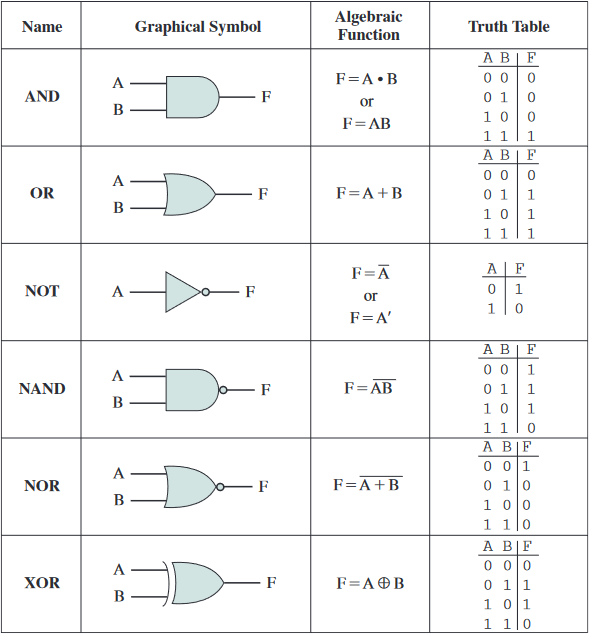
\includegraphics[width=300px]{assets/gates.png}
				\centering
				\caption{Figure of gates and their logical operation}
			\end{figure}
			These gates only have two output and one output except the NOT gate, but any number of inputs is possible and some gates may have two outputs where one is negated.\\
			When designing af circuit the fewer amount of gates the simpler and to complete possible operation the following set combinations are possible:
			\begin{itemize}
				\item AND, OR, NOT
				\item AND, NOT
				\item OR, NOT
				\item NAND
				\item NOR
			\end{itemize}
			When writing circuit, it can be done in two forms, sum of products, where product expression are multiplied, and product of sums (POS) where sum are multiplied.\\
			Both forms may not be the most simple form, but SOP uses only NAND, NOT and OR gates and POS uses only OR, AND, and NOT.\\
			To simplify a circuit there are different methods
			\begin{itemize}
				\item Algebraic simplifications - This can be done with indentities, which can simplify the expressions
				\item Karnaugh Maps - k-maps are a method which can help simplifying which variables are the out depended upon
			\end{itemize}
			
			\subsection{Karnaugh maps}
				This method works by taking 2 to 4 variables from a truthstable or function. They are then setup in a grid such all posibilities are accounted for.\\
				So for one side describing one variable there are 2 possibilites and a row which describes two variables there will be 4 possible outcomes.\\
				For each row/column combination the function or truthtable are used to determine if the cell is 0 or 1.\\
				Afterwards each 1 is circled in groups of powers of 2, so 1,2,4,8 or so on. A circle can not be cross or contain 0.\\
				For each circle the depending non changing variables are used in an and form and may be negated if the input was a consisten 0.\\
				For each circle the found AND expression is added with or to eachoter.
				\begin{figure}[h!]
					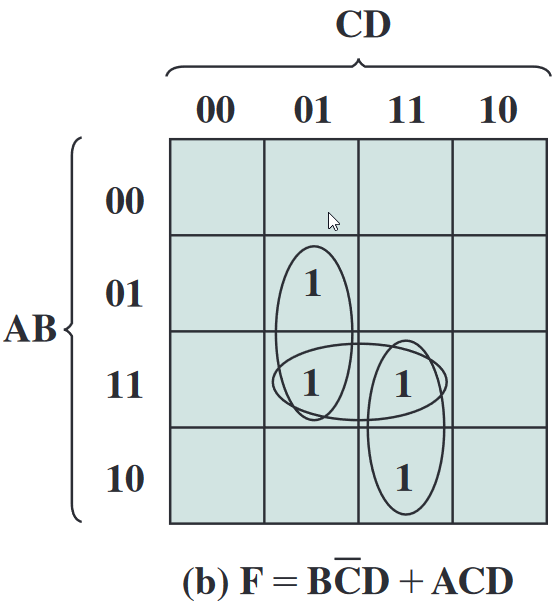
\includegraphics[width=200px]{assets/kmap.png}
					\centering
					\caption{Example of kmap and the output function}
				\end{figure}
			\subsection{Quine-McCluskey method}
				This is a more suitable method for SOP which have more than 4 variables.\\
				The method works by first creating a table with each collection of products on each row and in every column is the variables and in each cell are the needed value for the term to turn true.\\
				The table is then ordered such the row with most 0's is at the top at the row with most 1's are at the bottom.\\
				Then every row is compared to every row starting at the top, and if a row exist with only one column difference, the difference variable is eliminated and the rest of the variables are added to a new list.\\
				Then every element in the list is done with same procedure, and new found objects are added to the list. Then the same step is repeated with every new element until there is no new elements.\\
				Then every elment from the list is added to a table as rows and the original terms are added as columns.\\
				Then an X is placed in every cell where the row product is contained in the column. Then circle every X which is alone in a column, and square every X which are in a row with a circle.\\
				Those rows with a marked X are now needed for the minimal expression.
				\begin{figure}[h!]
					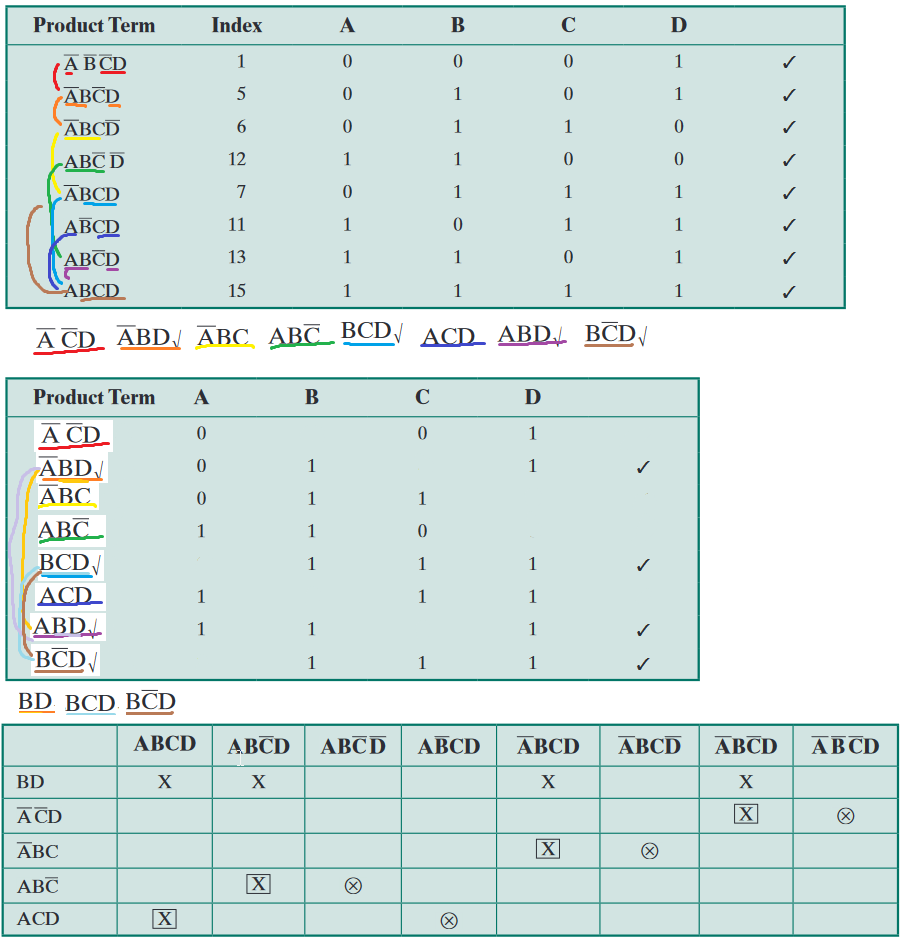
\includegraphics[width=300px]{assets/quine-McCluskey.png}
					\centering
					\caption{Example of the method on \\$F=ABCD+AB\overline{C}D+AB\overline{C}\overline{D}+A\overline{B}CD+\overline{A}BCD+\overline{A}BC\overline{D}+\overline{A}B\overline{C}D+\overline{ABC}D$\\
					Which result in the list $F=AB\overline{C}+ACD+\overline{A}BC+\overline{AC}D$}
				\end{figure}
			\subsection{Circuits}
				\subsubsection{Multiplex}
					Multiplex is a circuit of which a number of inputs label D0,D1,...,DN is wired to an output F.\\
					To controle which input determine the F value, the required number of selection inputs are used called S1,S2...,SN.\\
					So for a 4 input it would require two S inputs.\\
				\subsubsection{Decoders and encoders}
					A decoder is a circuit with a number of output lines, with only one asserted at the time.\\
					In general a decoder has $n$ input and $2^n$ outputs and can be usefull for writting a specific sequence of bits according to a simple code.\\
					An encoder will then be the inverse of the decoder.
				\subsubsection{Read-only Memory}
					As in the name this is memory, which can only be read from and are not programmable.\\
					This is implmented using a decoder and a set of OR gates.\\
					This is done by the a number inputs representing the placement of data and the OR gates each give out the value at the address.
				\subsubsection{Sequential circuits}
					Unlike combinational circuits as above a sequential circuits ouputs are depending on current inputs and the current state.\\
					The most simple form is a flip-flop, which is able to store one bit of data.\\
					There are different types of flip flops with different properties
					\begin{figure}[h!]
						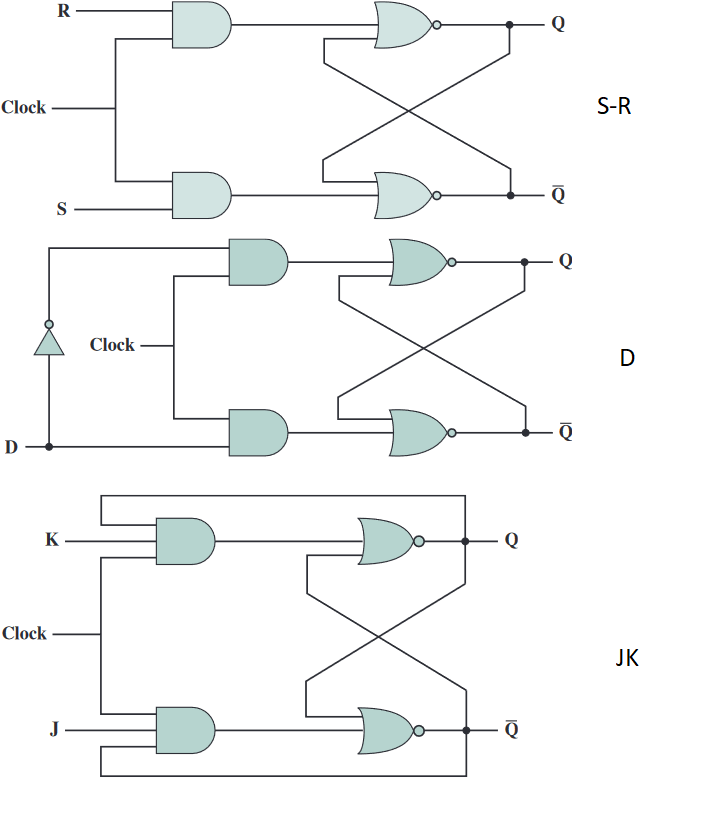
\includegraphics[width=300px]{assets/flipFlops.png}
						\centering
						\caption{Different types of flip flops}
					\end{figure}
					The SR flip flop can not have both S and R be 1 but is the most simple, with a on (S) and off (R)\\
					The D flip flop has a single switch for both on and off\\
					The JK flip flop can have both inputs be 1 and will simply result in Q being 0\\
					These flips flops can then be made in parrallel forming a register, or by as a shift register which has flip flops in series and are sending data down the series at each clock cycle with only input at the front.\\
					Another use case is a series of flip flops which creates a ripple counter or assyncronous counter, which when incrementet the effect ripples through all the other flip flops.\\
					Synchronous counters have the clock going into every flip flop. It can be observed that when counting in binary the first bit, simply flips on every count, the next bits flips when the right bit is 1.\\
					\begin{figure}[h!]
						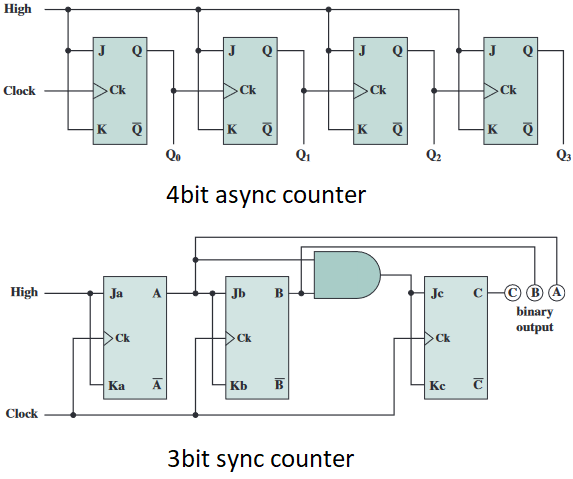
\includegraphics[width=300px]{assets/counters.png}
						\centering
						\caption{Two implmentations of binary counters}
					\end{figure}
				\subsubsection{Programmable logic devices}
					PLD are general-purpose chips.\\
					There are different types of PLD
					\begin{itemize}
						\item PLA - Programmable logic array, is circuit which allows a number of inputs in both normal and negated form, which goes into an array of and gates, which output are wired up to an OR array into the outputs. This takes advantage of SOP binary form
						\item FPGA - Field programmable gate array, is a circuit consisting og a logic block, which are programmable using flip flops, I/O blocks and interconnect which connects the I/O block to the internal logic blocks
					\end{itemize}
	\section{Instruction sets}
		\subsection{Machine instructions}
			A machine instruction consist of the following:
			\begin{itemize}
				\item Operation code - the code which describe the operation to be performed called opcode
				\item Source operand reference - The operation may one or more source reference for the operation
				\item Result operand reference - The reference to the result of the operation if it exist
				\item Next instruction reference - The reference which hold the next instruction for after the execution
			\end{itemize}
			The next instruction reference and result reference can reference memory in different sources:
			\begin{itemize}
				\item Main or virtual memory
				\item Processor register - in some cases one or more registers may contain memory addresses which can be reference by the register name
				\item Immediate - The reference may be contained in the current instruction
				\item I/O device 
			\end{itemize}
			When referencing instruction the opcode is most often represented as abbreviation called mnemonics, such as ADD\\
			Instructions can be of the following types
			\begin{itemize}
				\item Data processing - Artihmetid and logic instructions
				\item Data storage - movement of data from and to registers and memory locations
				\item Data movement - I/O instructions
				\item Control - Test and branch instructions
			\end{itemize}
			Instructions may be designed to use 
			\begin{itemize}
				\item 0 references - This will then use the stack for references
				\item 1 referenece - Performs the instruction on and saves in a common accumulator register or something alike which the instruction is used upon 
				\item 2 references - Performs the instruction and saves it in the first register
				\item 3 references - Performs instruction and first two references and saves in the last reference
			\end{itemize}
			When designing a set of instruction there are multiple questions have to be considered
			\begin{itemize}
				\item Operation repertoire - How many and which operations should be in the set
				\item Data types - Which data types should be avaliable
				\item Instruction format - Instruction lengthm number of addresses, size of varius field and so on
				\item Registers - Number of registers which should be referenceable and what their use should be
				\item Addressing - In which mode an address of an operand is specified
			\end{itemize}
		\subsection{Types of operands}
			For numbers there are 3 different types 
			\begin{itemize}
				\item Binary integer or binary fixed point - The classic integer in binary form
				\item Binary flaoting point - here the first bit mean the sign(1 = negative) the nest 8 bits are the exponent and the next 23 are the mantisse for the 32 bit version
				\item Packed decimal - used to avoid a lot of conversion, such every decimal is represented with 4 bits, and (1101) means - and (1100) means +
			\end{itemize}
			For representing characters 8 binary bits can be used with standards by ASCII, whcih dictates what the different binary combination represent.\\
			The x86 can deal with data types of 8 (byte), 16 (word), 32 (doubleword), 64 (quadword), and 128 (double quadword)\\
			ARM processors support data types of 8 (byte), 16 (halfword), and 32 (word) bits in length.\\
		\subsection{Types of operations}
			A useful and typical categorization is the following: 
			\begin{itemize}
				\item Data transfer - Calculate the memory address based on address mode, if virtual translate to real memory, detemine if data is not cached and issur a command to the memory module.
				\item Arithmetic - Different kind of matematic operations and may include data movement for the operation
				\item Logical - Logical operations such as XOR, right shift, left shift or rotate on binary data
				\item Conversion - Conversion between binary and decimal aswell as operation conversion between 8 bit and such
				\item I/O - Instructions for data movement in and out of the system
				\item System control - Privelege function often reserved to operation system, such as alter register control or modifying storage protection key.
				\item Transfer of control - Operations for changing execution with: branching on condition (if and loops), skip on condition (skip out loop or flow), call a block of code and return to current code (function calling) is done by calling it and pushing parameters and return to stack in a stack frame. 
			\end{itemize}
			When using conditions it refers to one of the architectures flags, which may be raised during instructions.\\
			For x86 the call specificly does
			\begin{itemize}
				\item Push the return point on the stack
				\item Push the current frame pointer on the stack
				\item Copy the stack pointer as the new value of the frame pointer
				\item Adjust the stack pointer to allocate a frame
			\end{itemize}
			This can be done manually by instructions or by the ENTER instruction though it takes 10 cycles instead of 6.\\
			MMX instructions are also exclusive to x86 and are instruction which can operate on multiple smaller data set by combining them into 32 or 64 bit chunks.\\
			This allows the instruction to work in parrallel on things like image processing where pixels are gathered in larger chunks.\\
			
	\section{Addressing modes and Formats}
		\subsection{Adressing modes}
			Adressing modes are different methods of getting an address which can be send to the accumilator.\\
			Most often a system implements two modes and the selected method is either in the opcode or in the memory field.\\
			\begin{figure}[h!]
				\centering
				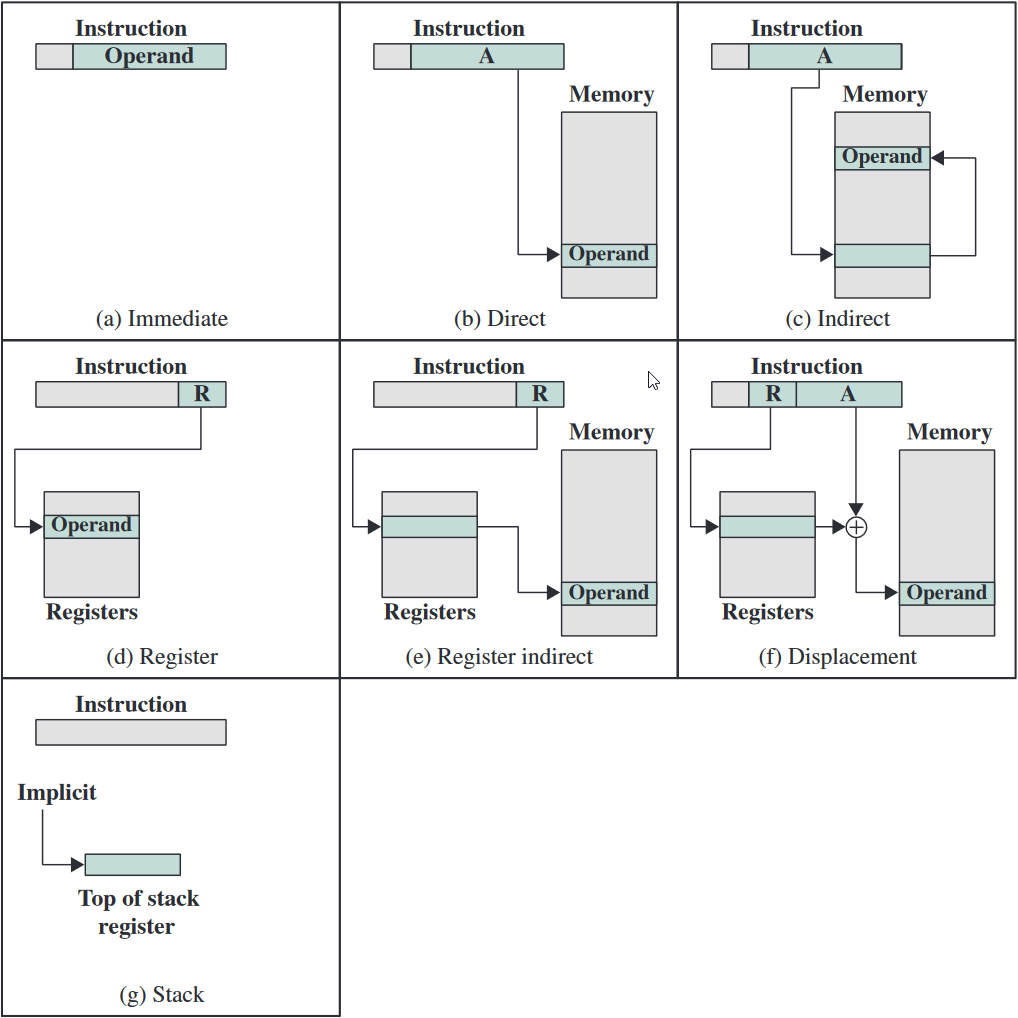
\includegraphics[width=300px]{assets/addressingModes.png}
				\caption{Illustrations of addressing modes}
			\end{figure}
			\begin{itemize}
				\item Immediate - The address is in the instruction, needs little memory but has size of address is limited to operand
				\item Direct - The instruction contains a memory location which value is the address, memory location is limited to operand size.
				\item Indirect - The instruction contains memory locations which contains memory location of which value is the address, first operand location is then low such it can contain a higher memory location
				\item Register - Same as direct but the operand refers to a register instead, registers are faster in case of reuse and requires a smaller address
				\item Register inderect - Same as indeirect but with registers
				\item Displacement - Operants are both a register address and a value which is added to the register value to find memory location containing address.
				\item Stack - Instead of instruction including a memory reference the stack is used to operate
			\end{itemize}
			Displacement can be used in different ways
			\begin{itemize}
				\item Relative - The register used is the program counter, such the memory location is relative to the current with the offset of the other operand.
				\item Base register - Uses the base registers value added with the other operand
				\item Indexing - Register contains offset and other operand is memory location, often used for loops, and autoindex may be enabled where it automaticly in a cycle increment.
			\end{itemize}
			 For autoindex, the new index is saved in the memory location, this is either done before preindexing or after the indirection it is postindexing.
		\subsection{Addressing in x86}
			\begin{figure}[h!]
				\centering
				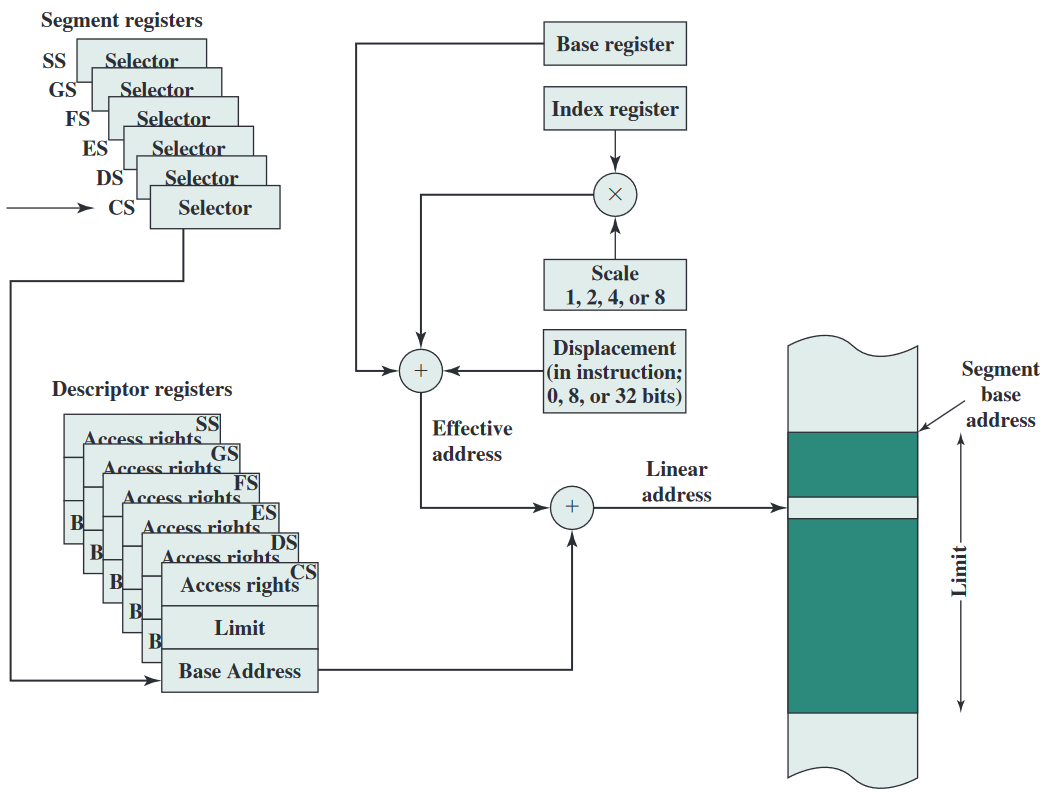
\includegraphics[width=300px]{assets/addressingModesCalculation.png}
				\caption{Addressing modes in x86 and how it is calculated}
			\end{figure}
			In x86 there are segment registers, these registers holds an index of the descriptor registers.\\
			The descriptor registers hold 3 values: Access right to the data, how much data there is and where the first part of the data is located.\\
			In addition there is a base register and index register.\\
			For register operand mode - either a 32 bit register, 16 bit register or 8 bit reguster can be used for data tranfer, aruthmetic and logical instructions.\\
			Displacement mode are not often used due to the long length up to 32 bits and are mostly used for global variables.\\
			For the rest if the addressing modes the memory location is referenced by the segment and the offset in the segment.\\
			Displacement mode with base is used for local variables, index of arrays and large record pointers.\\
		\subsection{Addressing in ARM}
			On arm there are three alternatives to indexing due to no index register being a thing.\\
			Offset - The instruction holds the offset as well as the register with the address.\\
			Preindex and postindex are offset but with the writing to the register either pre or post indexing.\\
		\subsection{Instruction formats}
			The length of an instruction is determined by a lot of factors, the longer the easier to program but more space.\\
			The length should be equal to memory-transfer or a multiple the length to ensure integral nnumber durin a fetch cycle.\\
			The length should also be optimized to be shorter due to memory most often being a bottlenect in speed. \\
			The instruction length should also be a multiple of 8 due to the character length, and how that relates to the word length such a word contain an integral number of characters.\\[4mm]
			The allocation of bits is also determined by multiple factors\\
			The more opcodes the more readable code and often less code, but som opcodes may be determined by the operands also.\\
			The amount of registers also affect the amount of bits required to describe a register. The ideal amount is found to be between 8 and 32.\\
			These registers can also be in sets such they can be determined with smaller amount of bits ex 2 sets of 8 requires 3 bits of data.\\
			The operands also need a good amount of data for addresses, not directly addresses but rather a big range for the displacement.\\
			Variable length instruction are variable length in the bit allocation in instruction which solves some of the many problems but requires more complexity in the processor and multiple instruction may be fetched at once.\\
			\subsubsection{x86 instruction format}
				\begin{figure}[h!]
					\centering
					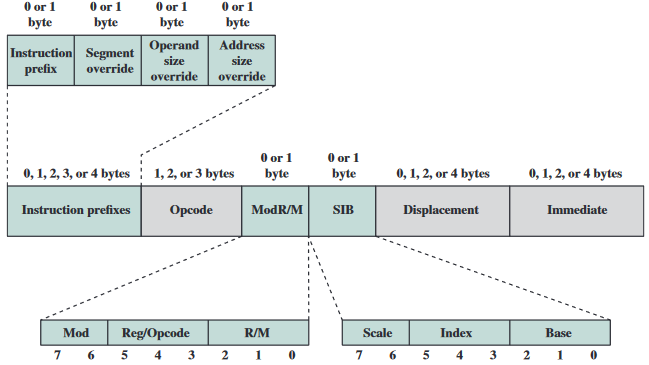
\includegraphics[width=300px]{assets/x86instructionFormat.png}
					\caption{x86 instruction format and it lengths}
				\end{figure}
				\begin{itemize}
					\item \textbf{Prefixes}
					\item Instruction prefixes - There are two avaliable prefixes, LOCK which ensures exclusive use of shared memory in multiprocessor envirements, and repeat prefixes which can be on of 5
					\begin{itemize}
						\item REP - repeats instruction until register CX is equal to zero
						\item REPE/REPNE - repeats until value of ZF flag
						\item REPZ/REPNZ - repeats until RCX, ECX or CV is equal 0
					\end{itemize}
					\item  Segment override - Overrides which segment register an instruction should use
					\item Operand size - Switches between 16 or 32 bits operands
					\item Address size - Switches between 16 or 32 bit address generation
					\item \textbf{Instruction}
					\item Opcode - 1 - 3 bytes of length may also include bits about: if data is byte- or fullsize, direction of data operation, immediate data field must be sign extended
					\item ModR/M - The location of the first operand (address mode or register) and the location of the second operand (a register) if required by the instruction. Or an extra bit for the opcode (opcode extension)
					\item SIB - If a specified address mode need more data the SIB contain: The scale field for scaled index (2 bits), index field (3 bits) for index register and base field (3 bits) for base register.
					\item Displacement - If displacement addressing mode is used, an 8-, 16-, or 32-bit signed integer displacement is specifed
					\item Immediate - Provides the value of an 8-, 16-, or 32-bit operand
				\end{itemize} 
			\subsubsection{ARM instruction format}
				\begin{figure}[h!]
					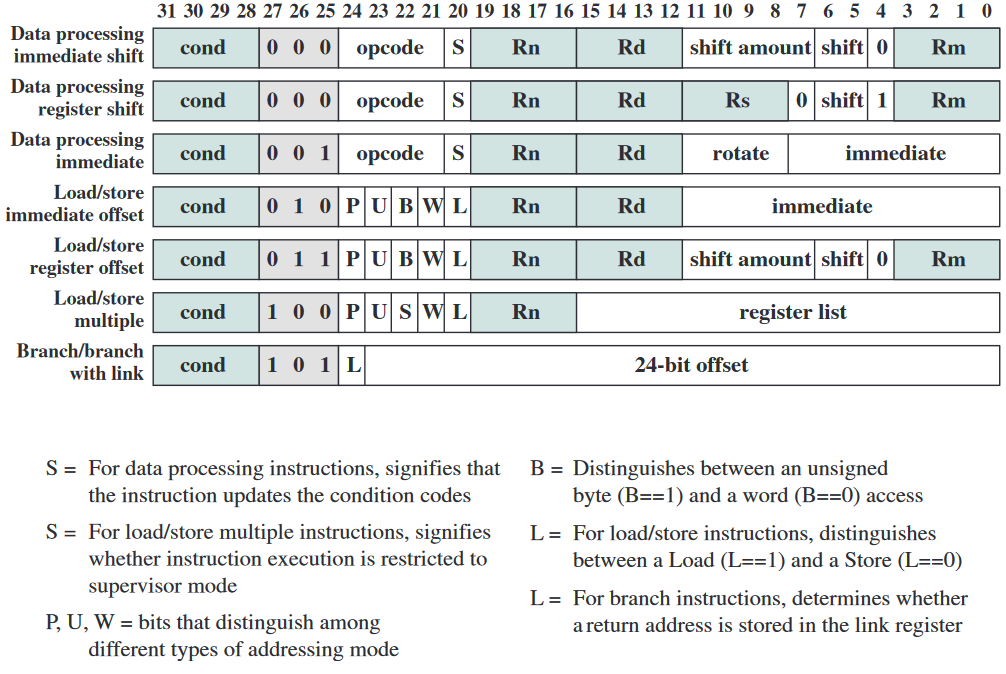
\includegraphics[width=300px]{assets/ARMInstructionFormat.png}
					\centering
					\caption{ARM instruction formats}
				\end{figure}
				\begin{itemize}
					\item Immediate constants - 8 bit constant value which can be rorated by 4 bit to create constants
					\item Thumb instruction set - A subset of instruction which have been decreased to 16 bit instead of 32 bit. This is done by
						\begin{itemize}
							\item Thumb instruction are unconditional, so the conditional field is not used and all arithmetic thumbs update the conditions flag, so not flag bits are needed
							\item The limited amount of opcodes only require 2 bits and 3 bit type field
							\item Thumb instructions only references registers r0 to r7 so only 3 bit is required
						\end{itemize}
					\item Thumb-2 instruction set - This is the bridge between ARM and thumb instruction which makes it possible to combine both instruction for more compact and performed code
				\end{itemize}
	\section{Assembly language concepts}
		Assember - compiler for assembly to object code\\
		Linker - Combines one or more files containing object code into a single loadable file or executable code\\
		Loader - Copies an executable into memory for execution\\
		Object code - Step between assembly and executable code
		Symobilic program - A static somewhat like assembly language with static memory\\
		Assembly uses symbolic addresses for data for non static references.\\
		The downsides of writing in assembly instead og high level language
		\begin{itemize}
			\item development time takes much longer
			\item Reliability and security are lower due to no compiler which can warn or throw errors of bad or unsecure code
			\item Debugging and verifying take longer due to more code resulting in more places it can go wrong
			\item Maintainability is low due to the often spaghetti like structure of assembly
			\item Protability is only on same platform
			\item HLL language have access to use intrisc functions so assembly is not required for device drivers and other system code
			\item Compilers are so good now that it often harder to write better assembly than the compiler
		\end{itemize}
		But there are upsides
		\begin{itemize}
			\item A compiled assembly code can be verified
			\item To create a compiler assembly is required
			\item Embedded systems may not be able to have a compiler and therefore need all code in assembly
			\item Hardware drivers and system code are often easier to program with assembly due to hll's not having access to hardware or registers or so on
			\item Accessing instructions that are not accessible from hhl
			\item Code size are often smaller with self written assembly
			\item Writing in assembly makes it possible to optimize more in speed than a compilers general optimization
		\end{itemize}
		\subsection{Assembly language elements}
			An assembly statement consist of: label, mnemonic, operand and comment
			\begin{itemize}
				\item Label (Optional) - Equivalent to address used for code references
				\item Mnemonic - Name of operand or function , symbolic name representing an opcode
				\item Operand(s) - zero or more operands may be given representing either a immediate value, a register value or a memory location
				\item Comment (Optional) - Text which are ignored by help the programmer in x86 it starts with a semicolon
			\end{itemize}
			When referencing data in operands there are different methods as discussed. \\
			For register addresses the register name is used.
			\begin{figure}[h!]
				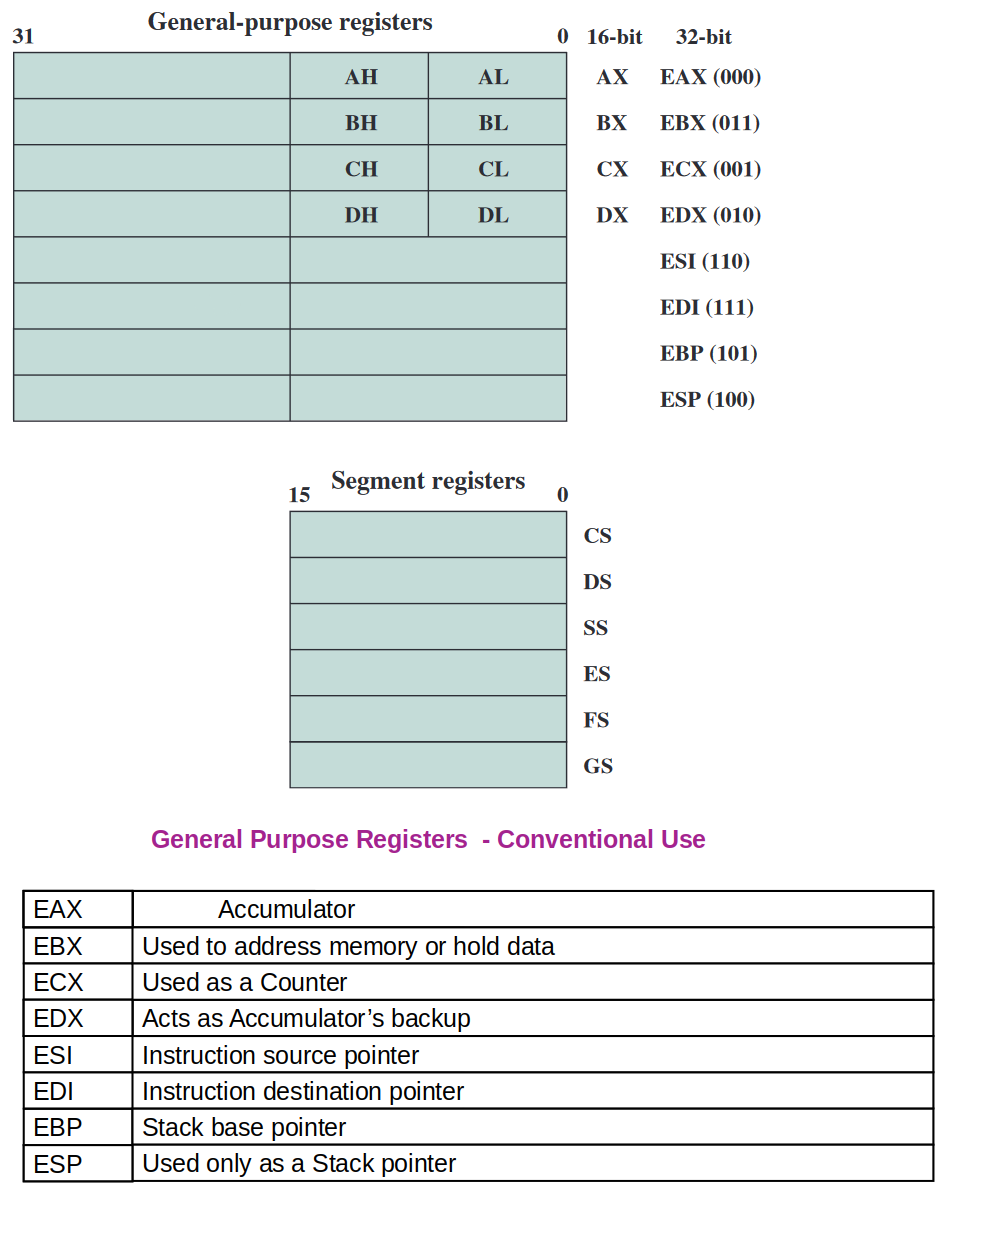
\includegraphics[width=300px]{assets/x86Registers.png}
				\centering
				\caption{x86 register names and their uses}
			\end{figure}
			For immediate addressing uses an indication that the value is encoded. Examples are H for hexadecimal, B for binary and decimal has no suffix\\
			Ex. 100B is read as a binary value\\
			For direct addressing expressed as a dispalcement from the DS segment.\\
			\subsubsection{Pseudo-instructions}
				Pseudo instruction are not x86 machine instruction but are still placed in the instruction field.\\
				\begin{figure}
					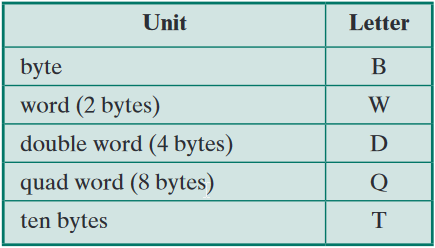
\includegraphics[width=200px]{assets/assemblyDirectives.png}\\
					\includegraphics[width=400px]{assets/x86Directives.png}
					\caption{Directives unit and letter and whtat the different pseudo instruction do}
					\centering
				\end{figure}
			\subsubsection{Macro definitions}
				Macros are a subroutine of code, and can be used multiple times like a call instruction.\\
				The main difference is macro expansion which actually inserts the macro at every instance to get rid of overhead time of instruction switching.\\
				This will result in a larger code but more clean code. \\
				Therefore a macro should only be a small bit of code.\\
				Macros can both be defined on single lines as - \%DEFINE A(X) = 1 + 8 + X and then be referede to as - MOV AX, A(8)\\
				For a multiline macro \\
				\%MACRO <NAME> <number of params>\\
					PUSH EBP;\\
					SUB EBP, \%1 ; first parameter\\
				\%ENDMACRO\\
		\subsection{Types of assemblers}
			\begin{itemize}
				\item Coss-assembler - Runs on another computer host to then be transfered to the target machine
				\item Residen assembler - Host and target are the same
				\item Macroassembler - Allows the user to define sequences of instructions as macros
				\item Microassember - Used to write microprograms which define the instruction set for a microprogrammed computer
				\item Meta-assembler - Can handle multiple instruction sets
				\item One-pass assembler - Produces machine code from a single pass of the assembly code
				\item Two-pass assember - Makes two passes to produce machine code
			\end{itemize}
			Two pass works by first finding and creating a symbol table of all symbols and their given location counter (LC).\\
			In the second pass the following is done
			\begin{itemize}
				\item Transte the mnemonic into binary upcode
				\item Use opcode the analyze the instruction
				\item Translate each operand to appropriate register or memory code
				\item Translate immediate value to binary
				\item Translate labels reference to LC 
				\item Set any other bit given in the instruction
			\end{itemize}
			The assembler also has a zeroth pass where it reads all macros which are defined at the top, such it can expand on first pass.\\[4mm]
			For a one pass compiler the trouble is keeping reference while translating which is done by, when a new label is found the following is done
			\begin{itemize}
				\item Leaves the instruction operand field empty in the assmbled binary instruction
				\item The symbol used as an operand is entered in the symbol table and flaged as undefined
				\item The address of the operand field is added to a list of forward references associated with the symbol table entry
			\end{itemize}
		\subsection{Loading and linking}
			Linker - Finds references to other code or data and links the references between object code (non linked machine code)\\
			A linker which produces a single module from the main module and it references to other modules is called the linage editor\\
			Load-time dynamic linking keeps all references to external modules and in run time when the external module is used it is loaded into main memory and the reference is updates.\\
			This also makes the libraries updatable and be in files themselves, ex in windows they are in dynamical-link libaries (DLLs), but this can also lead to DLL hell where two executables expect two different version of the same DLL file.\\[4mm]
			Loader - loads the final machine code into main memory \\
			There is 3 types of loading
			\begin{itemize}
				\item Absolute loading - Requires all modules are in the same loacation in memory, and references are absolute, this has many disadvantages with everything having to be in main memory at once and the absolute nature makes it near impossible to make correct references
				\item Relocatable loading - Every reference is relative to some point in the program, such that point location is just added to every other reference
				\item Dynamic run-time loading - To ensure that the program has not been moved since first loading, the references is first calculated with the offset when the reference is needed
			\end{itemize}
	\section{Assembly language x86}
		A list of every instruction can be found \href{https://www.felixcloutier.com/x86/}{here}\\
		The structure using at\&t is mnemonic source, destination.\\
		The registers start with \% and litteral valeus start with \$\\
		For comments \# is used.\\
		For 64 bit instruction, the opcode ends in q
		\subsection{Directives}
			Directive are part of code to initialize data or write the code.\\
			There are 3 types of sections .text, .bss and .data\\
			.data is for storing data and .bss is for allocating data.\\
			.text is for the code and global variables.\\
			Other forms of directives are for storing or allocating data.\\
			This can be done by: .space <numBytes> (Byte 8, Word 16, Doubleword 32, Quadword 64, Doulbe quadword 128)\\
			Or with text and label: myString: .ascii "Hello World!"
		\subsection{Starting the code}
			The assembler looks for the start of the code by:\\
			\begin{lstlisting}[language={[x86masm]Assembler}]
section .text
	global _start
_start:
	...\end{lstlisting}
		\subsection{Registers}[h!]
			From the existing registers the same space is actually used.\\
			The different registers and their space can be seen in the figure.\\
			In some instructions two registers may be used for wider range indicated by reg1:reg2 ex: RDX:RAX
			\begin{figure}
				\centering
				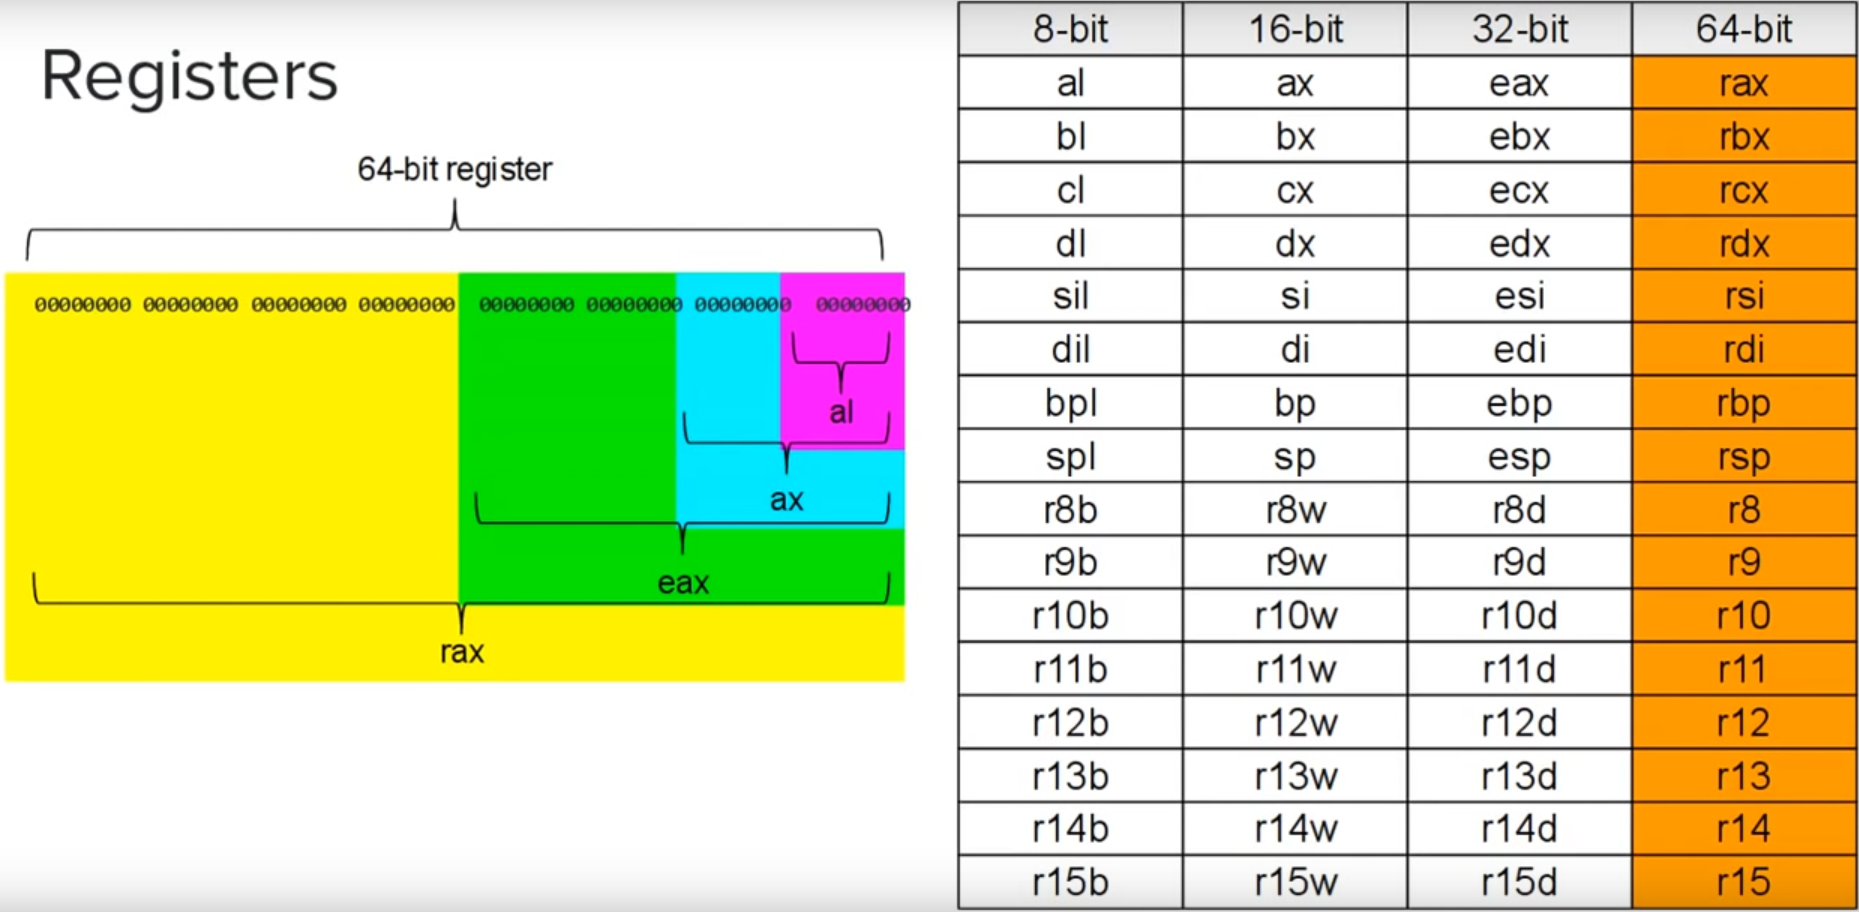
\includegraphics[width=300px]{assets/assemblyRegisters.png}
				\caption{The different registers in x86 assembly}
			\end{figure}
			\begin{itemize}
				\item RAX - accumilator for arithmetic operaions
				\item RBX - Base, holding a pointer to data
				\item RCX - Counter used in shift/rotate instructions and loops
				\item RDX - Data, used in arithmetic operations and I/O operations
				\item RSI - Source index, a pointer to data source in stream operations
				\item RDI - Destionation index, a pointer to data destination
				\item R8-R15 - New registers in 64 bit
				\item RSP - Stack pointer, points to top of stack
				\item RBP - Strack frame base, pointer to base of current stack frame
				\item RIP - Instruction pointer
			\end{itemize}
		\subsection{System calls}
			To make system calls the call and its arguments are putted into the following registers.\\
			\begin{itemize}
				\item ID - rax
				\item 1 - rdi
				\item 2 - rsi
				\item 3 - rdx
				\item 4 - r10
				\item 5 - r8
				\item 6 - r9
			\end{itemize}
			Every system call and their ids can be found \href{https://filippo.io/linux-syscall-table/}{here}.\\
			When every value is set the instruction 'syscall' can be called.\\[4mm]
			
			To end a program a exit system call is made with argument 0 symbolising the error code.\\
			\begin{lstlisting}[language={[x86masm]Assembler}]
section .text
	global _start
_start:
	movq $60, \%rax \#exit id is 60
	movq $0, \%rdi
	syscall \end{lstlisting}
		\subsection{Jumps}
			First the instruction cmpq <arg1> <arg2> is ran to set the flag\\
			Then one of the follwing condiiton jumps can be made
			\begin{itemize}
				\item je: $arg1\; ==\; arg2$
				\item jne: $arg1\; !=\; arg2$
				\item jg: $arg1\; <\; arg2$
				\item jge: $arg1\; <=\; arg2$
				\item jl: $arg1\; >\; arg2$
				\item jle: $arg1\; >=\; arg2$
			\end{itemize}
		\subsection{Stack and function calls}
			The stack goes from higher address to lower address.\\
			So when a new thing is pushed on the stack the RSP is decreased by 8 for each stack.\\
			When a function is called the stack is used in the following order to create a stack frame.
			\begin{itemize}
				\item Argument in reverse order
				\item Current instruction pointer 
				\item Local variables created in function
			\end{itemize}
			The called function is responsible for popping off the local variables and instruction pointer.\\
			The calling function has to pop the arguments.\\
			For first 6 integer/pointer arguments are in registers\\
			RDI, RSI, RDX, RCX, R8, and R9\\
			If more arguments are needed to stack is used.\\
			RAX is used for return value.\\
			For saving old register values they may be pushed to stack before beginning to function call.\\
			To call a function: call <label>\\
			And to return back from call: ret
	\section{Computer Arithmetic}
		The core of the computer is the arithmetic unit (ALU)\\
		Representing positive or negative a fixed number a bits is used to represent the number and the right most bit is a sign bit.\\
		This causes some drawbacks, mainly arithmetics are not as simple and checking for zero is also not as easy.\\
		\subsection{Sign-magnitude representation}
			The left most bit represent the sign if 1 then it is negative if 0 then positive.\\
			Drawbacks are bad arithmetic and hard to check for zero.
		\subsection{Twos compliment}
			Twos compliment counter act this by positive must the first bit be 0.\\
			Twos compliment of size $n$ is defined such if the most significant bit is 1, $2^n$ is subtracted to make it more simple.\\
			When negating twos compliment the most significant digit is flipped.\\
			The two edge cases 0 negation and the largest number negation, here a carry has to be remembered an used.\\
			\subsubsection{Twos compliment arithmetic}
				Doing addition is the same as binary, but the two most significant bits are not added rather XOR'ed\\
				For subtraction a negation is done and then an addition\\
				The addition is therefore done by a single addition unit taking two registers, saving the result in one of them or a third register, and indicate a possible overflow in a flag.\\
			\subsubsection{Twos compliment multiplication}
				For multiplication $n\times m$ bits, the $n$ bits are run through for every itteration a shift right of $m$ is done. If the bit itteration in $n$ is 1, $m$ is added to the summation.
				For multiplication of twos compliment, the multiplicand is in register $M$, multiplier in $Q$ and two extra registers are needed $A$ with start value of 0, and a single bit register we call $Q_{-1}$ to represent it being to the right of itteration of $Q$.\\
				Then $Q$ is itterrated through and looking at both $Q_i$ and $Q_{i-1}$.\\
				If the two bits differ then, if $Q_{i-1}$ is 1 then $M$ is added to $A$, and if $Q_{i-0}$ is 0 then $M$ is subtracted from $A$.\\
				If the two bits are the same, or an addition/subtraction is done, then $A$ and $Q$ is cyclic shifted to the right as one unit, and $Q_{-1}$ is what would have shifted into -1 \\
				This is repeated $n$ times where $n$ is the length of the multiplier.\\
				The result will be $AQ$.
				\begin{figure}[h!]
					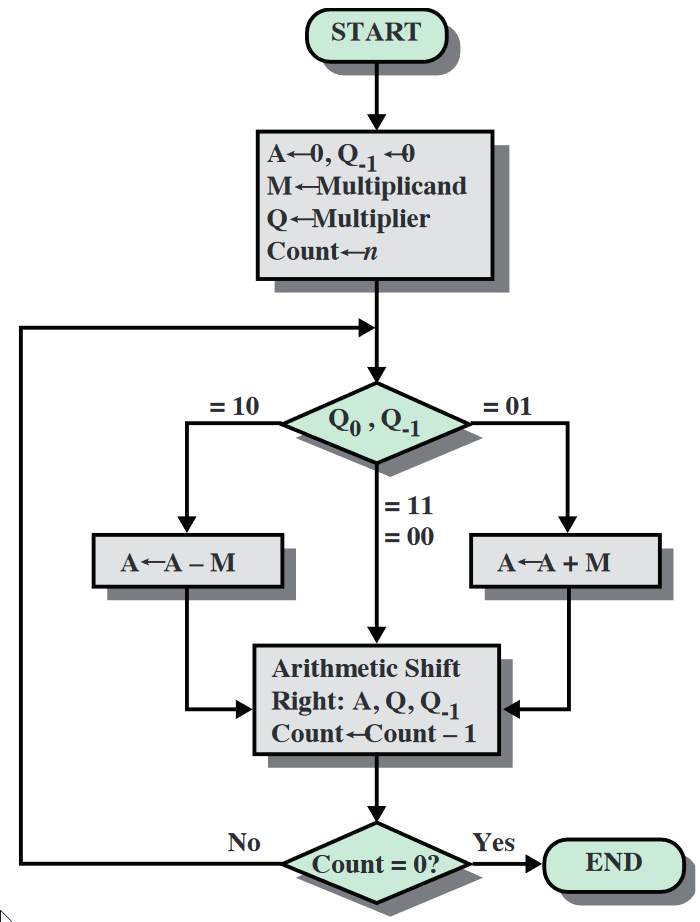
\includegraphics[width=200px]{assets/twosComplimentMultiplication.png}
					\centering
					\caption{Twos compliment multiplication diagram}
				\end{figure}
			\subsubsection{Twos compliment division}
				For division it differs not far, where $M$ is the divisor, $Q$ is the divident and a summation register $A$ with initial value 0.\\
				First $A$ and $Q$ is cyclic shifted left as one unit\\
				Then $M$ is subtracted to $A$.\\
				If $A$ is larger than zero (rightmost bit is 0) then set $Q_0=1$ otherwise set $Q_0=0$ and add $M$ to $A$.\\
				The remainder will be in $A$ and the quotient is in $Q$.
				\begin{figure}[h!]
					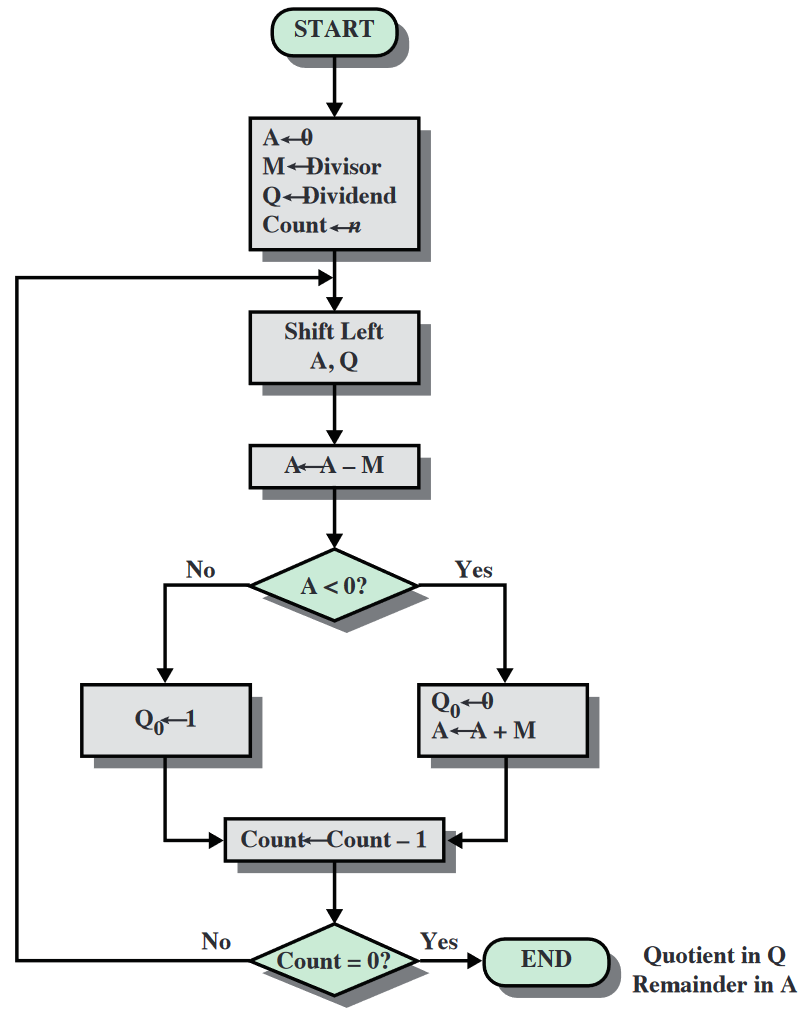
\includegraphics[width=200px]{assets/twosComplimentDivision.png}
					\centering
					\caption{Twos compliment division diagram}
				\end{figure}
		\subsection{Floating-point representation}
			For a typical 32 bit format of a floating point will be\\
			1 bit for sign,\\
			8 bits for exponent,\\
			23 bits for mantissa\\
			$sign 1.mantissa\cdot 2^{exponent}$\\
			For 64 the exponent is 11, and 128 15bits\\
			The exponent has a default bias being the negative value of half the range.\\
			This giving the values:
			\begin{figure}[h!]
				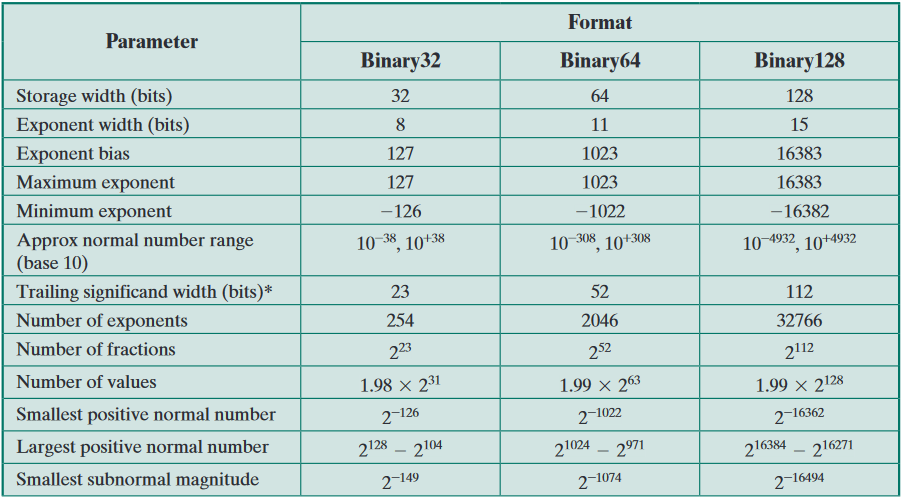
\includegraphics[width=300px]{assets/floatingPointLimits.png}
				\caption{Limits for the different floating point formats}
				\centering
			\end{figure}
			It can here be seen that the density of representable numbers is lower on higher numbers.\\
			When working with floating-point arithmetic one of the follwing may happend
			\begin{itemize}
				\item Exponent overflow
				\item Exponent underflow ending up being reported as 0
				\item Significand underflow/overflow ending up rounding such nothing really is changing
			\end{itemize}
			Subtraction and addition can be split into four groups
			\begin{itemize}
				\item Check for zeros - Change sign if subtraction, and check if one is equal to 0 such the result can be returned
				\item Align the significands - The lower number is shifted to the right and exponent is incremented, such the least significant bits are may lost
				\item Add or subtract the signifands - If overflow/underflow occur the exponent is either incremented or decremented
				\item Normalize the result - left shift until the left most digit is not zero and decrementing the exponent
			\end{itemize}
			\begin{figure}[h!]
				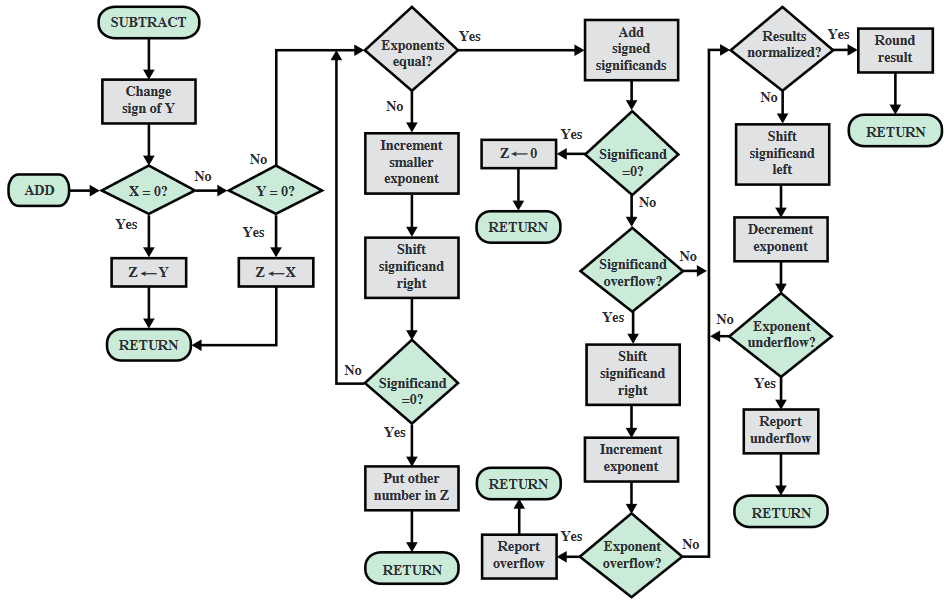
\includegraphics[width=300px]{assets/floatingpointAddSub.png}
				\centering
				\caption{Floating point addition and subtraction diagram}
			\end{figure}
			Multiplication
			\begin{itemize}
				\item Check for zeros
				\item Exponents are added together
				\item Significands are multiplied as normal integers
				\item Normalize the result
			\end{itemize}
			\begin{figure}[h!]
				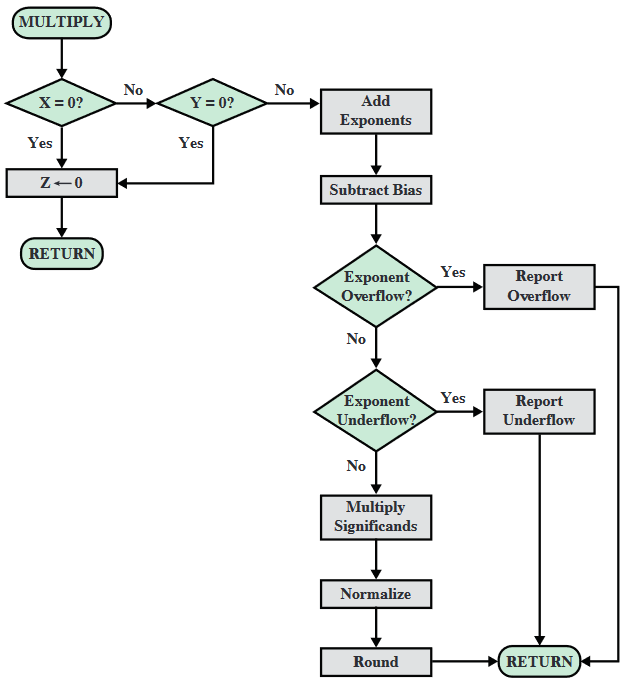
\includegraphics[width=300px]{assets/floatingpointMulti.png}
				\centering
				\caption{Floating point multiplication diagram}
			\end{figure}
			Pretty much the same for division, but instead exponents are subtracted and significands are divided as normal integers.\\
			Guard bits are extra zeros added to the end of the significant, such at left shift there will be less lost of significant bits.\\
			When the result is put into the given format rounding may be needed, there are 4 different approaches
			\begin{itemize}
				\item Round to nearest representable number, does require some extra statement for the exact between of two representable numbers, standard is towards even
				\item Round towards $+\infty$
				\item Round towards $-\infty$
				\item Round towards 0
			\end{itemize}
			 
		
			
\end{document}
